%	(step vs. move) 
%	Too much background on search which is not linked back. Introduction gives only context. Abstract gives concrete results (including what it means).
%	Check is meta-cognition could be error-monitoring. See lit.
%	Add the metacognition term in title, abstract and conclutions
%	Add conclusions add the end of solution progress.
%	Raise questions in introduction that I'm going to answer later
% 	Make sure all figures have the same font sizes 
%	Make Figure:Puzzle smaller and nicer(better colors).
%	Move figure descriptions to captions.
%       distinct between rt before and rt after a move
%       calculate rt per path
%       p11: see how we can describe the "bursts" effect with http://www.sciencedirect.com/science/article/pii/S0165027006004742
%       Examine the difference in human solution length per instance. See if we can explain this with a model/heuristics.
% 	Real results - real-dist
% 	real results - total expansions per instance 
% 	Look at all instances, measure mistakes per instance. Show that there is something else that determines mistakes
% 	Show that path length/mistakes/rt/ corresponds to weight and not to noise
%	Make sure error bars are always across subjects.
%	Consider saying combinatorial tasks instead of planning. 
%	Talk about the lack of understanding. - that people are relatively good at this, but suboptimal

%%
% Annual CCN conference
% Sample LaTeX Two-Page Summary -- Proceedings Format
% based on the prior cognitive science style file
\documentclass[10pt,letterpaper]{article}

\usepackage[font=small,labelfont=bf]{caption}
\usepackage{ccn}
\usepackage{subfig}
\usepackage{pslatex}
\usepackage{apacite}
\usepackage{graphicx}
\usepackage{multirow}
\graphicspath{ {figures/} }
 


\title{Suboptimality and Metacognition in Human Sequential Planning}
 
\author{{\large \bf Zahy Bnaya (zahy.bnaya@nyu.edu)} {\large \bf Wei Ji Ma (weiji.ma@nyu.edu)} \\
Center For Neural Science and Department of Psychology, New York University\\
}

\begin{document}

\maketitle

\section{Abstract} {\bf
 
People are naturally good (but suboptimal) at sequential planning tasks such as navigation or puzzles. While suboptimal planning can be done efficiently in various ways, we still do not understand properly the mechanisms and processes underlying human behavior. In this paper we report preliminary results that characterize human behavior on a combinatorial planning task. We show patterns in solution lengths, solution progress, and response times. We identified a pattern of "bursting" behavior in the response times within a solution. Subjects perform a slow move, followed by a series of multiple rapid moves. This might indicate that subjects spend time planning on some choices and then executing their plan fast on others. This burst pattern repeats itself multiple time within a solution which might also suggest that people perform partial search, which is a powerful method to find suboptimal solutions. We found that response times are affected by the distance to the goal and the step number within the solution. Additionally, our results suggest that people have some degree of knowledge about how well they are doing in the task. Subjects react slower when they are about to make mistakes and tend to forfeit a task only when they drifted far away from the goal. 



%The abstract should be identical to the text version submitted in the webform and should not exceed 1,500 characters, including spaces and any special characters. The       abstract should thus be relatively short. Aim for 150 words.
%Max length is 200 words. Arbitrarily long German words like "Donaudampfschiffartskapit\"an" are not encouraged.
%CCN has an interdisciplinary audience. Hence a good abstract should
%(a) give context about what the problem is and why it matters
%(b) give the contents and explain what was done and what was found
%(c) give a clear conclusion including what we learned and how it changes
%the way we think about the universe.
}

\begin{quote}
\small
\textbf{Keywords:} 
decision making; planning; heuristic search
\end{quote}


\vspace{-0.7cm}
\section{Introduction}
\vspace{-0.3cm}
In sequential planning the goal is to find a strategy that accomplishes a desired goal, given the initial state of the world and a set of possible actions. The common approach in Artificial Intelligence is to perform \emph{search} in the state space~\cite{russell1995modern}. Search methods can be \emph{optimal}, in the sense that the resulting strategy achieves the goal with minimal number of steps~\cite{korf1985depth,hart1968formal}. Planning tasks can quickly become difficult due to combinatorial explosion, therefore there is also a myriad of suboptimal search techniques such as performing hierarchical search~\cite{holte2005hierarchical} or performing partial search that finds an approximate or incomplete strategy~\cite{korf1990real,koenig2001agent}. Suboptimal techniques deal with memory or computational limitations in a principled way by efficiently sacrificing optimality for tractability and speed, usually without dramatically damaging the solution quality. Humans are not optimal planners but show good abilities in some planning tasks~\cite{acuna2008bayesian,pizlo2005solving,macgregor1996human,van2016people}. The mechanisms behind human behavior and how people balance solution quality and speed are still not well understood. In this paper we present preliminary results that characterize human behavior. 



%Check if minimal is really minimal. Use 770x320
%TODO: Cut black lines.
%TODO: Change color schemes
%TODO: Fix labels 
%TODO: Switch sides

\begin{figure}[ht]
	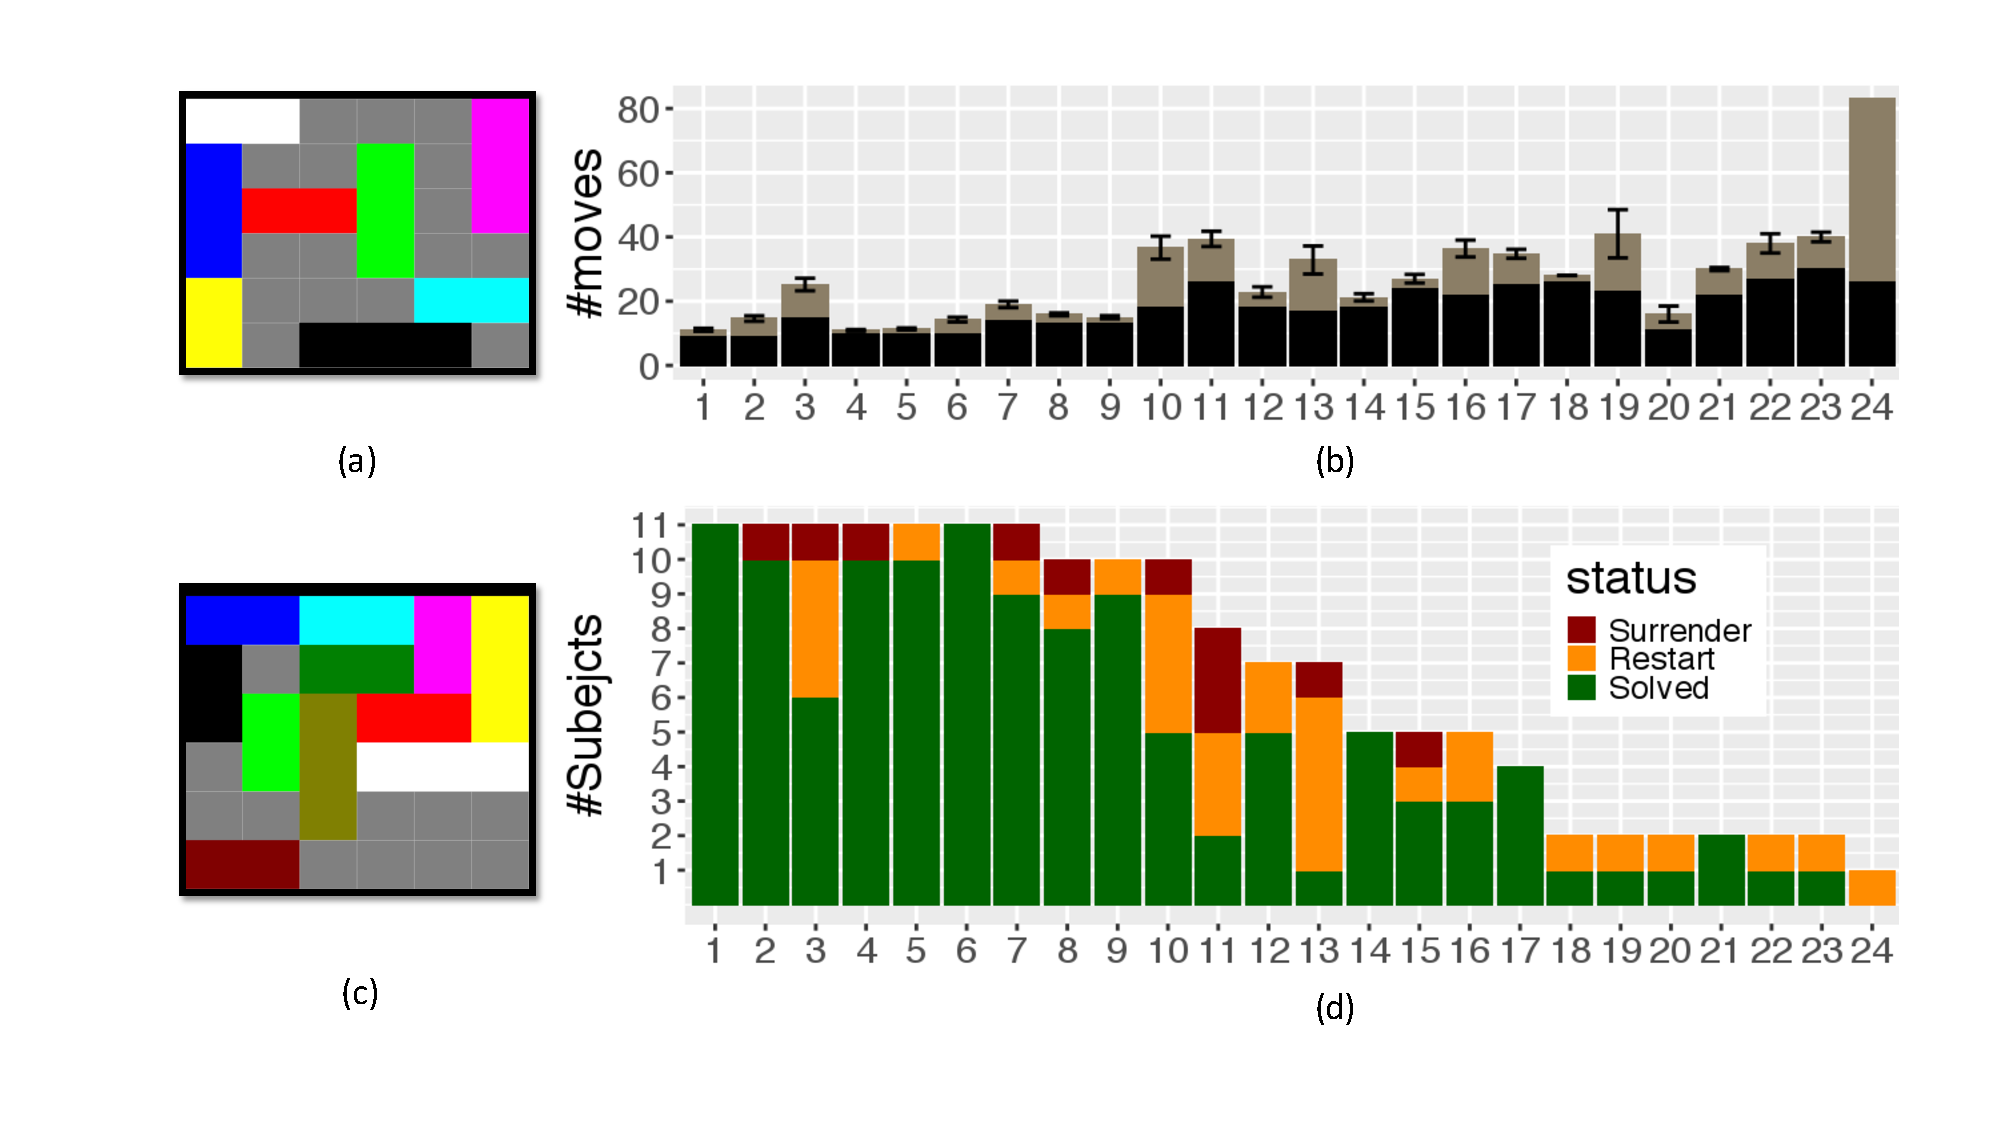
\includegraphics[width=0.5\textwidth]{puzzle_j}
\vspace{-0.5cm}
\caption{ (a) mean number of moves performed to solve each puzzle (minimal solution length in black). (b) number of subjects who decided to surrender, restart (at least once), or solved the puzzle on the first trial; two puzzles we used in our experiment, easy puzzle-1 (c) and more difficult puzzle-16 (d)}
	\label{fig:puzzle}
\vspace{-0.5cm}
\end{figure}


\vspace{-0.5cm}
\section{Methods}
\vspace{-0.1cm}
11 subjects solved up to 40 puzzles of the game \emph{rush-hour}\footnote{\url{www.thinkfun.com/play-online/rush-hour/}}. Rush-hour is a planning game, shown to be in PSPACE-complete~\cite{flake2002rush}. The puzzle (Figure~\ref{fig:puzzle}(a,c)) consists of a set of cars located on a 6 x 6 grid. Cars are oriented horizontally or vertically and can move only on the direction of orientation. The goal is to find a sequence of moves, such that the red car moves to the right edge of the screen. Subjects used a mouse and a keyboard to move the cars around. We imposed a time limit of 30 minutes. The order of puzzles was chosen arbitrary, but with a tendency to increase in difficulty (Figure~\ref{fig:puzzle}(b)). At any point, subjects were allowed to \emph{surrender} and move to the next puzzle or \emph{restart} the current puzzle by pressing a key on the keyboard. We recorded response times. 

\vspace{-0.1cm}
\section{Experiment results}
\vspace{-0.1cm}
All errors are SEMS across subjects.
Subjects completed on average $13.6 \pm 0.9$ puzzles (min=6, max=24), with $41.6\%\pm 2.4\%$ more moves than the minimal solution. Out of 231 solutions, 45 were optimal. Subjects tended to avoid the restart and surrender buttons. Five subjects surrendered, and only three surrendered more than once. Eight subjects chose to restart at least one puzzle~(Figure~\ref{fig:puzzle}(c)).

\subsubsection{Response times}
Response times was correlated with the step number ($-0.216\pm0.011$, Spearman, Figure~\ref{fig:rt}(a)). Subjects spent a factor of $5.67 \pm 0.18$ more time before their first decision than the rest of steps, possibly to devise a plan.  

\subsubsection{Burst analysis}
As a preliminary test of whether response times follow a "burst" pattern we performed a median split into \emph{fast} and \emph{slow} moves of each solution attempt. We define a \emph{burst} of size $n$ has a sequence of a slow move followed by $n-1$ fast moves. We found that subjects mean \emph{burst length} was $28.7\% \pm 0.5\%$ longer than the expected mean burst length of random ordering. This suggests that subjects tend to have a slow decision followed by a burst of fast decisions. Possibly for the sake of planning and executing the plan respectively. 
Response times were also correlated with the distance from the goal ($0.211\pm0.019$; Figure~\ref{fig:rt}(b)).
However, we could also detect a quadratic relationship ($R^2=0.041\pm0.004$). Subjects tend to react faster when they were closer to the goal, probably because finding plans for easier states is faster. Response times were also faster when subjects were far away from the goal. This can be explained by subjects switching to a fast strategy when the complete plan seems difficult to find. (link to partial search, link to meta-cognition).
\begin{figure}[t]
\vspace{-0.03cm}
	\centering
	\subfloat[][]{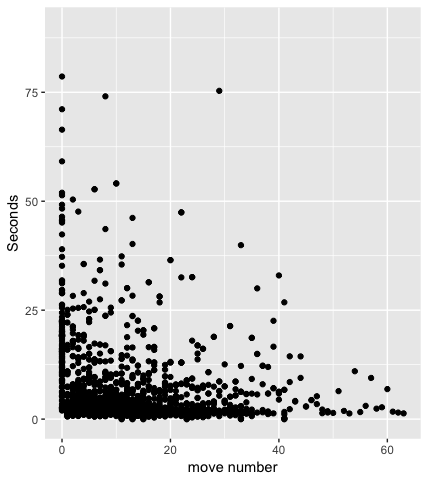
\includegraphics[width=0.5\linewidth]{p3_1}}
	\subfloat[][]{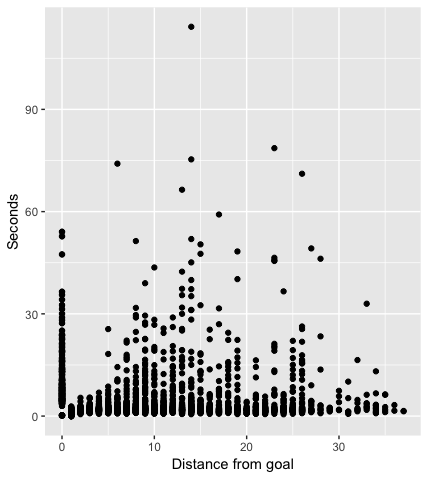
\includegraphics[width=0.5\linewidth]{p25}} 
\vspace{-0.1cm}
	\caption{Response time in relation to (a) move number (b)  distance from goal} 
\vspace{-0.55cm}
	\label{fig:rt}
\end{figure}

\begin{figure}[!h]
\begin{center}
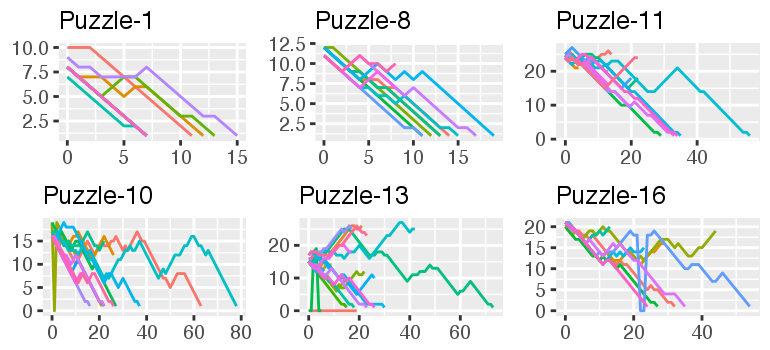
\includegraphics[width=0.44\textwidth]{p6_1}
\end{center}
\vspace{-0.6cm}
\caption{Solution Progress in example puzzles. A complete solution reaches distance zero, other solution paths either restarted or surrendered. Easier puzzles showed less variability (the top row) than difficult puzzles (bottom row).} 
\vspace{-0.2cm}
\label{fig:progress}
\end{figure}

\begin{figure}[h]
\vspace{-0.5cm}
	\centering
	\subfloat[][]{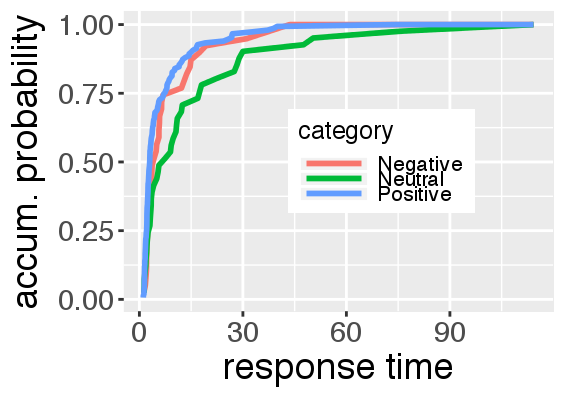
\includegraphics[width=0.32\textwidth]{p16_1}}
	\subfloat[][]{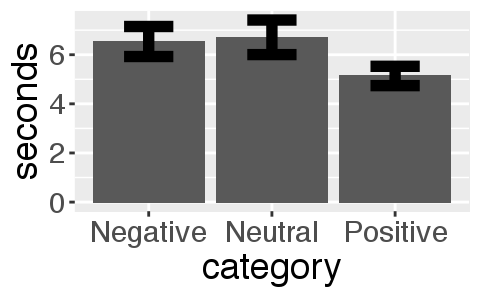
\includegraphics[width=0.18\textwidth]{p16_3}}
	\vspace{-0.1cm}
	\caption{(a) CDF of one subject rt per category (b) Mean response times for move category} 
	\label{fig:rt_cat}
\vspace{-0.5cm}
\end{figure}

\vspace{-0.2cm}
\subsubsection{Solution progress}
We calculate the progress of solutions by examining the minimal distance to the goal after each move~(Figure~\ref{fig:progress}). Subjects generally recover from errors and move towards the goal. Variability in progress increased on difficult puzzles(show or delete). Usually subjects decided to surrender when they were X steps further from the initial state, and restart when they where Y steps far away from the initial state. This suggests that subjects had some indication of their solution progress. In order to check if subjects are aware to their progress, we categorize moves into \emph{positive} moves, if the move progressed closer to the goal,\emph{negative} (moved away from the goal), or \emph{neutral} (kept the same distance). In total, 2,891 moves were positive, 702 negative and 816 neutral. The mean numbers of moves per subject were $262.8 \pm 23.6$ (positive), $74.1 \pm 8.0$ (negative) and $63.8 \pm 7.6$ (neutral).
We tested whether response times vary on different categories of moves. We found that the mean response time of positive moves is different than that of negative moves ({\bf p-val $< 0.001$}), the mean response time of positive moves is different than that of neutral moves ({\bf p-val $= 0.004$}). We did not find evidence that negative and natural moves are different.
We used wilcoxon paired test.

\vspace{-0.3cm}
\section{Discussion and conclusion}
\vspace{-0.15cm}
%structure - finding, conclution, intepretation (join findings where possible)
We present preliminary results and show that people are suboptimal with sequential planning task. Subjects spend more time on earlier steps within a plan and on decisions which were objectively wrong. This suggests that subjects had some sense of of how well they were doing. Another indication for the same phenomenon is that subjects decide to restart or surrender only when they were getting far away from the goal.  We further examined the patterns in response times and found that subjects act in an interleaved periods of fast and slow moves. This might suggest that people are performing partial search, a powerful suboptimal method. An additional indication for partial search is that subjects tend to decide faster not only when they are close to the goal but also when they are far away from the goal and cannot find a complete plan. For future work we plan to fit models of human behavior, examine additional behavioral aspects and perform a larger experiment.




%%The entire contribution of a short summary submission (including
%figures, references, and anything else) can be no longer than two
%pages. This short summary format is to be used for workshop and
%tutorial descriptions, symposia summaries, and publication-based
%presentation extended abstracts. Unlike submitted research papers,
%short summary submissions should \emph{not} begin with a separate
%abstract. Prior to the first section of the short summary, there
%should be the header ``{\bf Keywords:}'' followed by a list of
%descriptive keywords separated by semicolons, all in 9~point font, as
%shown above.
%
%The text of the paper should be formatted in two columns with an
%overall width of 7 inches (17.8 cm) and length of 9.25 inches (23.5
%cm), with 0.25 inches between the columns. Leave two line spaces
%between the last author listed and the text of the paper. The left
%margin should be 0.75 inches and the top margin should be 1 inch.
%\textbf{The right and bottom margins will depend on whether you use
%  U.S. letter or A4 paper, so you must be sure to measure the width of
%  the printed text.} Use 10~point Modern with 12~point vertical
%spacing, unless otherwise specified.
%
%The title should be in 14~point, bold, and centered. The title should
%be formatted with initial caps (the first letter of content words
%capitalized and the rest lower case). Each author's name should appear
%on a separate line, 11~point bold, and centered, with the author's
%email address in parentheses. Under each author's name list the
%author's affiliation and postal address in ordinary 10~point type.
%
%Indent the first line of each paragraph by 1/8~inch (except for the
%first paragraph of a new section). Do not add extra vertical space
%between paragraphs.
%
%
%\section{First Level Headings}
%
%First level headings should be in 12~point, initial caps, bold and
%centered. Leave one line space above the heading and 1/4~line space
%below the heading.
%
%
%\subsection{Second Level Headings}
%
%Second level headings should be 11~point, initial caps, bold, and
%flush left. Leave one line space above the heading and 1/4~line
%space below the heading.
%
%
%\subsubsection{Third Level Headings}
%
%Third level headings should be 10~point, initial caps, bold, and flush
%left. Leave one line space above the heading, but no space after the
%heading.
%
%
%\section{Formalities, Footnotes, and Floats}
%
%Use standard APA citation format. Citations within the text should
%include the author's last name and year. If the authors' names are
%included in the sentence, place only the year in parentheses, as in
%\citeA{NewellSimon1972a}, but otherwise place the entire reference in
%parentheses with the authors and year separated by a comma
%\cite{NewellSimon1972a}. List multiple references alphabetically and
%separate them by semicolons
%\cite{ChalnickBillman1988a,NewellSimon1972a}. Use the
%``et~al.'' construction only after listing all the authors to a
%publication in an earlier reference and for citations with four or
%more authors.
%
%
%\subsection{Footnotes}
%
%Indicate footnotes with a number\footnote{Sample of the first
%footnote.} in the text. Place the footnotes in 9~point type at the
%bottom of the column on which they appear. Precede the footnote block
%with a horizontal rule.\footnote{Sample of the second footnote.}
%
%
%\subsection{Tables}
%
%Number tables consecutively. Place the table number and title (in
%10~point) above the table with one line space above the caption and
%one line space below it, as in Table~\ref{sample-table}. You may float
%tables to the top or bottom of a column, or set wide tables across
%both columns.
%
%\begin{table}[!ht]
%\begin{center} 
%\caption{Sample table title.} 
%\label{sample-table} 
%\vskip 0.12in
%\begin{tabular}{ll} 
%\hline
%Error type    &  Example \\
%\hline
%Take smaller        &   63 - 44 = 21 \\
%Always borrow~~~~   &   96 - 42 = 34 \\
%0 - N = N           &   70 - 47 = 37 \\
%0 - N = 0           &   70 - 47 = 30 \\
%\hline
%\end{tabular} 
%\end{center} 
%\end{table}
%
%
%\subsection{Figures}
%
%Make sure that the artwork can be printed well (e.g. dark colors) and that 
%the figures make understanding the paper easy.
% Number figures sequentially, placing the figure
%number and caption, in 10~point, after the figure with one line space
%above the caption and one line space below it, as in
%Figure~\ref{sample-figure}. If necessary, leave extra white space at
%the bottom of the page to avoid splitting the figure and figure
%caption. You may float figures to the top or bottom of a column, or
%set wide figures across both columns.
%
%\begin{figure}[ht]
%\begin{center}
%\fbox{CCN figure}
%\end{center}
%\caption{This is a figure.} 
%\label{sample-figure}
%\end{figure}
%
%
%\section{Acknowledgments}
%
%Place acknowledgments (including funding information) in a section at
%the end of the paper.
%
%
%\section{References Instructions}
%
%Follow the APA Publication Manual for citation format, both within the
%text and in the reference list, with the following exceptions: (a) do
%not cite the page numbers of any book, including chapters in edited
%volumes; (b) use the same format for unpublished references as for
%published ones. Alphabetize references by the surnames of the authors,
%with single author entries preceding multiple author entries. Order
%references by the same authors by the year of publication, with the
%earliest first.
%
%Use a first level section heading, ``{\bf References}'', as shown
%below. Use a hanging indent style, with the first line of the
%reference flush against the left margin and subsequent lines indented
%by 1/8~inch. Below are example references for a conference paper, book
%chapter, journal article, dissertation, book, technical report, and
%edited volume, respectively.
%
%\nocite{ChalnickBillman1988a}
%\nocite{Feigenbaum1963a}
%\nocite{Hill1983a}
%\nocite{OhlssonLangley1985a}
%% \nocite{Lewis1978a}
%\nocite{Matlock2001}
%\nocite{NewellSimon1972a}
%\nocite{ShragerLangley1990a}
%
\vspace{-0.3cm}
\bibliographystyle{apacite}

\setlength{\bibleftmargin}{.125in}
\setlength{\bibindent}{-\bibleftmargin}

\bibliography{sequential_planning}


\end{document}
